\graphicspath{{02_literature_review/figures/}} % Location of the graphics files

\chapter{Literature Review}
\label{02_chp:literature_review}

Due to the foundational aspect of common grounding, there is a rich and diverse literature related to this topic. In this chapter, we first give an overview of the existing literature on common grounding (Section \ref{02_sec:common_grounding}). Then, we review the contemporary approaches to dialogue system engineering (Section \ref{02_sec:dialogue_systems}). Finally, we discuss the important links to the related (yet distinct) problem of symbol grounding (Section \ref{02_sec:symbol_grounding}).

\section{Common Grounding}
\label{02_sec:common_grounding}

In this section, we first give an overview of the theoretical foundations of common grounding, including the literature in philosophy, mathematical logic and psycholinguistics (Section \ref{02_subsec:theoretical_foundations}). Then, we review the computational models of common grounding in natural language conversations, including both formal and empirical approaches (Section \ref{02_subsec:computational_approaches}).

\subsection{Theoretical Foundations}
\label{02_subsec:theoretical_foundations}

The notion of common ground (or \textit{common knowledge}) was originally conceived by David Lewis \citep{lewis1969convention} to explain the nature of human \textit{conventions}. Conventions are the regularities in our behavior which we expect each of us to understand and follow: without them, we cannot account for our solutions to various \textit{coordination problems} \citep{Schelling1960}, from setting up daily meetings to communicating in natural language. In essence, \citeauthor{lewis1969convention} argues that such expectations can only be justified based on a certain level of common ground established within the community.

In later studies, common ground came to be recognized as ubiquitous and essential in various linguistic phenomena/competence, including presupposition \citep{stalnaker1978assertion}, definite reference \citep{Clark1981-CLADKA}, communication \citep{clark1996using} as well as first language acquisition \citep{clark2001grounding}.

But what exactly is common ground? Can it be defined formally, and do we know how exactly they are built up? The absolute answers may not be established yet, but there are three major approaches which account for these questions.\\

\noindent
\textbf{Epistemic Logic}\quad
The first approach is studied in the field of epistemic modal logic \citep{fagin2003reasoning}. To give a brief introduction, we consider $A$ to be the set of agents and $p$ to be a proposition. Then, using the modal operator $K_a$, we can represent the epsitemic state that ``an agent $a \in A$ knows $p$'' as $K_a\,p$. Similarly, we can represent the state that ``all agents in $A$ know $p$'' based on the operator $E_{A}\,p$ (which is equivalent to $\bigwedge_{a \in A} K_a\,p$). Finally, if we use the abbreviation $E_{A}^n\,p$ for $E_{A}\,E_{A}^{n-1}\,p$ (where $E_{A}^{0}\,p\,=\,p$), we can represent the state ``$p$ is \textit{common knowledge} among $A$'' based on the operator $C_{A}\,p$ (which is equivalent to $\bigwedge_{i=1}^{\infty} E_{A}^i\,p$).

The process of common grounding can be taken into account by using additional operators which represent the \textit{actions} or \textit{events} that cause the change in agents' epistemic states: such logical framework is known as dynamic epistemic logic \citep{van2007dynamic}. If we assume the agents to be perfectly logical reasoners, this framework allows for computing the exact set of common ground after each information update.

However, the formulations and assumptions in this approach may not be cognitively plausible. For instance, a literal interpretation of common knowledge imposes an infinite list of epistemic conditions to be checked \citep{Clark1981-CLADKA}, and humans may not be perfect logical reasoners either. This drawback makes the theory difficult to be applied in realistic settings, such as natural language dialogues.
\\

\noindent
\textbf{Shared Basis}\quad
The second approach defines common ground based on the notion of \textit{shared basis} \citep{lewis1969convention,Clark1981-CLADKA}. To be specific, this approach considers a proposition $p$ to be common ground among the agents i.f.f. there exists some state of affairs $b$ such that:

\begin{enumerate}
  \item Every agent has information of the basis $b$.
  \item $b$ indicates to every agent that every agent has information of $b$.
  \item $b$ indicates to every agent that $p$ holds.
\end{enumerate}

For instance, in a situation where agents are \textit{co-present} and \textit{co-observing} a house on fire, these state of affairs become the shared basis for the common ground ``there exists a house on fire''. This approach is more cognitively plausible because the infinite, recursive assessment of epistemic states is not required (as in the previous approach). Furthermore, the shared basis need not be represented symbolically and hence accounts for \textit{multi-modal} (non-linguistic) common grounding through gestures \citep{lascarides2009formal}, eye gaze \citep{nakano-etal-2003-towards} and other mediums that are commonly used in face-to-face interactions.

However, current approaches so far define common ground independently for each proposition $p$. Is it possible to define common ground (and common grounding) in its entirety, including their interrelationships and non-propositional knowledge? The last approach offers an interesting perspective which takes this into account.
\\

\noindent
\textbf{Situation Models}\quad
The last approach employs the concept of \textit{situation models}. Situation models are the mental representations of the state of affairs described in text or conversation \citep{zwaan1998situation}. For instance, there is empirical evidence in cognitive psychology that humans are sensitive to spatial layouts when comprehending stories \citep{GLENBERG198769} and constructs spatially coherent representations as they read along \citep{ferguson1994properties}. These studies suggest that comprehension of language is not merely an analysis of syntactic/semantic structures, but should rather be considered as construction of situation models coherent with the linguistic descriptions (e.g. in terms of spatial, temporal and causal dimensions).

Following this idea, \citet{pickering2004toward} consider common ground(ing) as the \textit{alignment} of situation models among the interlocutors. Based on this view, the process of common grounding does not require explicit reasoning of the epistemic states, as required in the previous approaches. Instead, they argue that such alignment proceeds mostly implicitly at various linguistic levels, including phonetic, lexical, syntactic and semantic representations. For instance, lexical entrainment naturally leads to aligned conceptualization, which is also in line with the theory of \textit{conceptual pacts} \citep{Brennan1996ConceptualPA}.

This approach has the advantage of representing the entire common ground as the \textit{aligned situation models}, which capture the holistic view of common ground (including their internal structures and non-linguistic knowledge). However, the lack of strict definitions and strong empirical evidence (e.g. on how situation models are actually aligned) potentially remain as its major challenges.\\

It is worth noting that our formalization of common grounding (Section \ref{01_sec:contributions}) is closest to the last definition by \citet{pickering2004toward}. However, we circumvent the difficulty of dealing with entire situation models by restricting our scope to \textit{entity-level alignment}, which keeps the task simple, well-defined and quantifiable.

\subsection{Computational Approaches}
\label{02_subsec:computational_approaches}

The previous section focused on the conceptual (\textit{epistemic logic}) or psychological (\textit{shared basis} and \textit{situation models}) foundations of common grounding. Unfortunately, they are not directly applicable for our practical goal of developing \textit{computational} models of common grounding through \textit{natural language} interaction.

\subsubsection{Formal Approaches}

To model common grounding in actual human conversations, \citet{traum1994computational} conducted a pioneering work based on a refinement of the contribution theory \citep{clark1989contributing}. To be specific, he defined a set of \textit{grounding acts} (such as \textit{initiate}, \textit{continue}, \textit{repair}, \textit{request repair} and \textit{acknowledge}) by taking into account the speech acts \citep{austin1962things,searle1969speech} relevant to common grounding. Based on these grounding acts, a finite state model is used to compute the transition of information in dialogue, until it reaches the final accepting state (and considered to be in common ground).

In subsequent works, the idea of this approach has been integrated with Discourse Representation Theory \citep{Kamp1981-KAMATO-2,kampreyle93} to represent the semantic (e.g. propositional) contents of common ground \citep{poesio1997conversational}. In Segmented Discourse Representation Theory \citep{asher2003logics}, \textit{rhetorical relations} are also taken into account to capture the implicit process of common grounding, e.g. through the initiation of the next relevant contribution. Such formal representations provide elaborate computational models of not only common grounding but natural language dialogue in general \citep{ginzburg2012interactive}.

However, formal approaches come with their own disadvantages. For instance, identifying the precise semantic representation of a dialogue is a challenging task requiring time and high expertise. They are also unable to capture various complexities in realistic dialogues, such as ambiguity and uncertainty in common grounding. Finally, they are not directly applicable to \textit{situated} dialogues involving rich non-linguistic contexts, such as vision and embodied environments.

\subsubsection{Empirical Approaches}

To overcome these limitations, recent works mostly focus on empirical methods and develop \textit{data-driven} models of common grounding. The primary step in this approach is to collect dialogue corpora: such attempts have originated in the HCRC Map Task Corpus \citep{anderson1991hcrc} and continued since then \citep{potts2012goal,tokunaga-etal-2012-rex,zarriess-etal-2016-pentoref}. Recent works often utilize crowdsourcing to collect diverse data at scale: notable works include the GuessWhat?! dataset \citep{de2017guesswhat}, MutualFriends dataset \citep{he2017learning}, PhotoBook dataset \citep{haber-etal-2019-photobook} as well as our own \citep{udagawa2019natural,udagawa2021maintaining}. As an illustration, we show an excerpt of the common grounding task from the PhotoBook dataset in Figure \ref{02_fig:photobook_sample}, where the human players try to identify the common images through dialogue.\footnote{Note that the players are indeed relying on \textit{entity-level alignment} to succeed in common grounding.}

\begin{figure*}[t!]
\centering
\includegraphics[width=\textwidth]{photobook_dataset_sample.pdf}
\caption{An excerpt from the PhotoBook dataset \citep{haber-etal-2019-photobook}. In this task, two human players are provided different combinations of images and try to find out whether the (bordered) images are in common or not.
}
\label{02_fig:photobook_sample}
\end{figure*}

The second step is employ machine learning \citep{murphy2012machine} to train the models based on the collected corpora, typically in an \textit{end-to-end} or fully data-driven manner. By leveraging the actual human dialogues, we can expect the models to learn fundamental strategies of common grounding (e.g. clarifications and elaborations) without expensive, potentially unreliable annotations. We can also expect the models to capture the ambiguity and uncertainty in common grounding owing to their high flexibility. Finally, this approach can naturally be applied in situated conversations, e.g. by treating multi-modal information in a unified manner based on neural networks \citep{GoodBengCour16}. We will explain the specific model architectures in Section \ref{02_subsec:models}.

Note that most of the existing common grounding tasks focus on closed domain, goal-oriented dialogues, including our collaborative reference tasks (c.f. Figure \ref{01_fig:contribution_overview}): this is for the sake of quantitative and objective evaluation based on the \textit{task success rates}, as we discussed in Chapter \ref{01_chp:introduction}. However, some recent works also attempt to model this in open domain, non-goal-oriented dialogues: for instance, \citet{cho-may-2020-grounding} developed a model of (single-turn) common grounding through creative improvisation of the next relevant contribution. While its evaluation remains an open challenge, this new approach sheds light on interesting potential applications, such as the development of more engaging, entertaining and coherent chat-bots.

\section{Dialogue Systems}
\label{02_sec:dialogue_systems}

In this section, we review the broader literature of dialogue system research in general. Unfortunately, most of the existing works do not specifically focus on common grounding: for instance, they do not require advanced common grounding skills nor enable direct evaluation/analysis of such abilities. However, understanding the broader literature is fundamental for common grounding research, since they provide crucial insights on the related problems and engineering solutions. Besides, it is important to place the role of common grounding in the general settings of dialogue, which will be one of the main focuses of this section.

\subsection{Tasks and Datasets}
\label{02_subsec:tasks_and_datasets}

Dialogue research is conducted under various motivations and practical goals: consequently, numerous tasks and datasets have been proposed in the existing literature. To make our review as inclusive as possible, we categorize them into the following 4 types: namely \textit{(traditional) task-oriented dialogues}, \textit{multi-modal dialogues}, \textit{non-cooperative dialogues}, and \textit{non-goal-oriented dialogues}.
\\

\noindent
\textbf{Task-Oriented Dialogues}\quad
Traditionally, the central motivation of dialogue system research has been a practical one: to develop industrial-level dialogue systems that can execute a variety of useful tasks. The expected tasks include booking a trip \citep{elasri2017frames} or recommending movies \citep{chen-etal-2019-towards} by interactively soliciting the user's preferences. Due to its practicality, many existing benchmarks and shared tasks have been focusing on such task-oriented dialogues \citep{henderson-etal-2014-second,budzianowski-etal-2018-multiwoz,lee2019multi}. Recent works propose valuable extensions as well, e.g. based on scalable task ontologies \citep{rastogi2020towards} and efficient domain adaptations \citep{shalyminov2020fast}

However, the underlying settings in these tasks remain mostly unchanged and do not require advanced common grounding. To be specific, they only need to deal with \textit{categorical} databases or knowledge graphs, which do not require semantic coordination from the ground up. For instance, continuous concepts like the price range would be discretized in advance (e.g. to ``cheap'', ``moderate'' and ``expensive''), so that they can avoid sophisticated common grounding and keep the tasks manageable. 

If we were to develop truly conversational and practical systems, we should start focusing on systems that can deal with more advanced settings, e.g. that can negotiate on the exact preferences on a \textit{continuous} scale. Without such ability, dialogue systems cannot adequately respond to the user's precise requests, e.g. in terms of the price range, location, atmosphere, and so on.\\

\noindent
\textbf{Multi-Modal Dialogues}\quad
Recently, increasing attention has been paid to multi-modal dialogues, especially those grounded in the visual modality \citep{das2017visual,de2017guesswhat,alamri2019audio}. These works lie at the intersection of computer vision (CV) and NLP, involving intricate cognitive reasoning \citep{zellers2019recognition} and spatio-temporal grounding (c.f. Section \ref{02_subsec:spatio_temporal_grounding}). Such extension to the visual modality is also useful in practice. For instance, \citet{moon-etal-2020-situated} proposed a dialogue task where the system can display and manipulate a shared screen with the user: this allows for better interaction and improved user experience, especially in shopping domains (e.g. for fashion and furniture) where item apperances play a key role.


However, it remains unclear to what extent existing tasks require precise dialogue understanding and spatio-temporal grounding. First, there are minimal linguistic analyses conducted on these datasets, and the complexities of the dialogue structures remain unrevealed. Secondly, there could be various sources of undesirable biases in realistic visual contexts \citep{goyal2017making,cirik-etal-2018-visual}, and the tasks may not necessarily require genuine intricate abilities. For instance, existing visual dialogue tasks may be largely solvable without taking into account \textit{dialogue history} \citep{agarwal-etal-2020-history}, contrary to the expectation when it was first proposed \citep{das2017visual}.

Therefore, we argue that more attention must be paid to the requisite skills of visually-grounded dialogues and their reliable evaluation. Common grounding and symbol grounding are the two central competence we focus on and address in this thesis.
\\

\noindent
\textbf{Non-Cooperative Dialogues}\quad
All of the previous tasks so far (including the common grounding tasks) have assumed that dialogue is \textit{cooperative}, i.e. the goals of the interlocutors are fully aligned. However, this may not necessarily be the case in general. Typical departures include the cases of negotiation \citep{lewis-etal-2017-deal,he-etal-2018-decoupling,li2020noncollaborative}, where the interlocutors' goals may be different or even conflicting (e.g. they must compete for a fixed amount of resource). Such situations may also arise when one needs to persuade the other to profit a third party \citep{wang-etal-2019-persuasion} or in the case of malicious scams where one is intending to deceive the other \citep{li2020noncollaborative}. On such occasions, the interlocutors need to exert complex reasoning skills and negotiation strategies to achieve their desired outcomes.

However, this does \textit{not} indicate that common grounding can be non-cooperative in such settings. On the contrary, we argue that fully cooperative common grounding plays a fundamental role in maintaining any type of conversation. Even in the case of negotiation, the interlocutors must cooperate and share (certain levels of) the same understandings to disagree, compromise, or take any extreme measures \citep{lewis1969convention,sacks1987preferences}. This suggests that we must take into account the collaborative aspect of common grounding, even if our goal was to study dialogues in non-cooperative settings.
\\


\noindent
\textbf{Non-Goal-Oriented Dialogues}\quad
Finally, we raise the category of \textit{non-goal-oriented} dialogues, typically referred to as chit-chats. The main objective of this research is to develop \textit{engaging} and \textit{coherent} chatbots that can handle a wide variety of topics, ranging from sports, politics to technology \citep{ram2018conversational}. One key factor that affects engagement is \textit{empathy}, the cognitive ability of understanding and acting on behalf of the user's emotional states. Microsoft XiaoIce, one of the world's most popular chatbots today, explicitly incorporates such empathetic mechanisms \citep{zhou2020design}. To assess and improve the consistency of chatbots, \citet{zhang-etal-2018-personalizing} proposed a dialogue setting where the interlocutors are provided artificial profiles to act in accordance to. In subsequent works, the profiles are extended to fictitious character settings and grounded in more open-ended text adventure games \citep{urbanek-etal-2019-learning}.

In recent years, there has been an impressive breakthrough on the model side based on gigantic-scale neural networks \citep{adiwardana2020towards,roller-etal-2021-recipes}. While they exhibit almost human-level performance under specific setups, they still do not possess the true competence of natural language conversation. To demonstrate this, \citet{benotti-blackburn-2021-grounding} raised an example dialogue with BlenderBot, the state-of-the-art chatbot from Facebook \citep{smith-etal-2020-put,roller-etal-2021-recipes}:

\ex.
\a. Human:\; Do you know Blender?
\b. BlenderBot:\; Yes, I've used it a little bit. I am not very good at it, though.
\c. Human:\; But I don't mean the 3D software.
\d. BlenderBot:\;  Oh, I see. Yeah, I know a little bit about it. What do you like to do with it?
\e. Human:\; I mean Blender, the chatbot. Have you used it?
\f. BlenderBot:\; Oh, yes, I have used it. I like to use it to make 3D models.

In this conversation, the human speaker clarifies that ``Blender'' refers to the chatbot and not the 3D software (c). Impressively, BlenderBot acknowledges its misunderstanding and makes a perfectly coherent recovery (d). However, in the last utterance (f), it turns out that BlenderBot had not actually resolved its misunderstanding and once again misinterprets ``Blender'' as the 3D software. 

This example demonstrates the lack of true common grounding capacity of modern chatbots: in this case, the ability of accurate \textit{entity-level alignment}. To realize truly engaging and coherent chatbots, we expect that more robust and reliable common grounding will be the key in non-goal-oriented dialogues as well.

\subsection{Evaluation Metrics}
\label{02_subsec:evaluation}

Evaluation plays a crucial role in the development of dialogue systems. The specific measures can vary depending on the task domain: for instance, the \textit{task success rate} may be the primary metric in task-oriented dialogues, \textit{each player's payoff} may be so in non-cooperative dialogues and \textit{user satisfaction} in non-goal-oriented dialogues. Such evaluation can be conducted either manually (e.g. based on questionnaires) or automatically (e.g. based on regressions from the relevant factors, \citealt{walker-etal-1997-paradise}).

There are also task agnostic approaches to dialogue evaluation. For instance, \textit{human-likeness} is usually a desirable factor in all types of dialogues. While this is relatively straightforward to measure manually based on human judgements, automatic evaluation of such quality remains an open challenge. For instance, reference-based metrics such as BLEU \citep{papineni-etal-2002-bleu} may not correlate with human evaluation \citep{liu2016}, and regression-based metrics such as ADEM \citep{lowe-etal-2017-towards} can easily be fooled by simple adversarial attacks \citep{sai2019re}.

For a comprehensive review of existing evaluation methodologies, we refer to a recent survey by \citet{Deriu2020SurveyOE}. However, throughout this thesis, we argue that the evaluation of dialogue systems should focus more on their \textit{abilities} \citep{Hernndez-Orallo:2017:MME:3110808} rather than the ad-hoc performance metrics (such as benchmark scores). This means that we should answer the following research questions through the design of dialogue tasks and evaluation metrics:

\begin{itemize}
	\item What are the specific abilities required to succeed in this task setting?
	\item Does the evaluation metric truly reflect such abilities?
\end{itemize}

In the field of psychometrics, these two questions roughly correspond to the concepts of \textit{validity} and \textit{reliability}, respectively \citep{cook2006current}. Unfortunately, current evaluation of dialogue systems often neglects the first question: for instance, it is not made clear what linguistic capabilities and strategies are required in a certain dialogue setting. Many works also fail to answer the second question: for instance, the existence of dataset biases makes the evaluation unreliable and unfaithful.

From this aspect, we hope this thesis contributes important insights on the requisite skills and evaluation of \textit{common grounding}, which should be taken into account in all types of dialogues (as discussed in Section \ref{02_subsec:tasks_and_datasets}).

\subsection{Model Architectures}
\label{02_subsec:models}

Finally, we give an overview of the mainstream architectures in dialogue system engineering. As briefly discussed in Chapter \ref{01_chp:introduction}, there are two major approaches in developing modern dialogue systems. In Figure \ref{02_fig:two_dialogue_systems}, we show an illustration of the two approaches from a recent survey paper \citep{gao2019neural}.\\

\begin{figure*}[th!]
\centering
\includegraphics[width=0.95\textwidth]{two-dialogue-system.pdf}
\caption{An illustration of the two mainstream architectures of data-driven dialogue systems from \citet{gao2019neural}.
}
\label{02_fig:two_dialogue_systems}
\end{figure*}

\noindent
\textbf{Traditional Dialogue Systems}\quad
The first approach is based on a pipeline/modular architecture, which has traditionally been used for task-oriented dialogue systems (Figure \ref{02_fig:two_dialogue_systems}, top). In this framework, the \textit{natural language understanding (NLU) module} is first applied to the user utterance to extract relevant information, typically in a structured format. This can be as simple as a pair of user intent and named entities \citep{Gupta2006TheAS} or more complex graph-based representations which capture anaphora, relations, and utterance ambiguity \citep{kollar-etal-2018-alexa}. Next, the \textit{dialogue state tracker} integrates the extracted information with the previous dialogue state to update the current state. Dialogue states are often represented based on the \textit{frame} structure (i.e. slot-value pairs), possibly one for each domain under control \citep{elasri2017frames}. In a recent approach, these are extended to executable data-flow graphs \citep{andreas-etal-2020-task} which are much more general and expressive. Based on the updated dialogue state, the system can optionally query the database for necessary information \citep{dhingra-etal-2017-towards} and the \textit{dialogue policy module} determines the content of the system response \citep{takanobu-etal-2019-guided}. Finally, the \textit{natural language generation (NLG) module} either retrieves an appropriate response template \citep{yan2016learning} or generates the surface form conditioned on the determined content \citep{wen-etal-2015-semantically}.\\

\noindent
\textbf{End-to-End Dialogue Systems}\quad
In the second approach, dialogue systems are typically trained in a fully data-driven manner based on \textit{end-to-end} neural networks. Under this setting, dialogue modeling is often treated as a type of \textit{(conditional) language modeling} problem \citep{vinyals2015neural}: conditioned on the input sequence of dialogue history, compute the probability of the next dialogue responses.

Formally, let $D = \{d^1, d^2, ..., d^{|D|}\}$ be the dialogue corpus containing the dialogue sequence $d^i = \{x^i_1, x^i_2, ..., x^i_{|d^i|}\}$. We generally consider each element of the dialogue sequence $x^i_t$ to be a \textit{token}: however, it can also be in the unit of the whole \textit{utterance} \citep{serban2016hierarchical}. Given $D$ as the dataset, the learning objective is to find the model parameters $\theta$ that minimize the sum of negative log probabilities (or equivalently, maximize the product of total probabilities)
%
\begin{equation}\label{eqt:sequence_to_sequence}
L(\theta) = \sum_{i = 1}^{|D|} \sum_{t = 1}^{|d^i|} - \log p(x^i_t | x^i_{<t}, \theta)
\end{equation}
%
where $x^i_{<t} = \{x^i_1, x^i_2, ..., x^i_{t-1}\}$ (which represent dialogue history).

\begin{figure*}[th!]
\centering
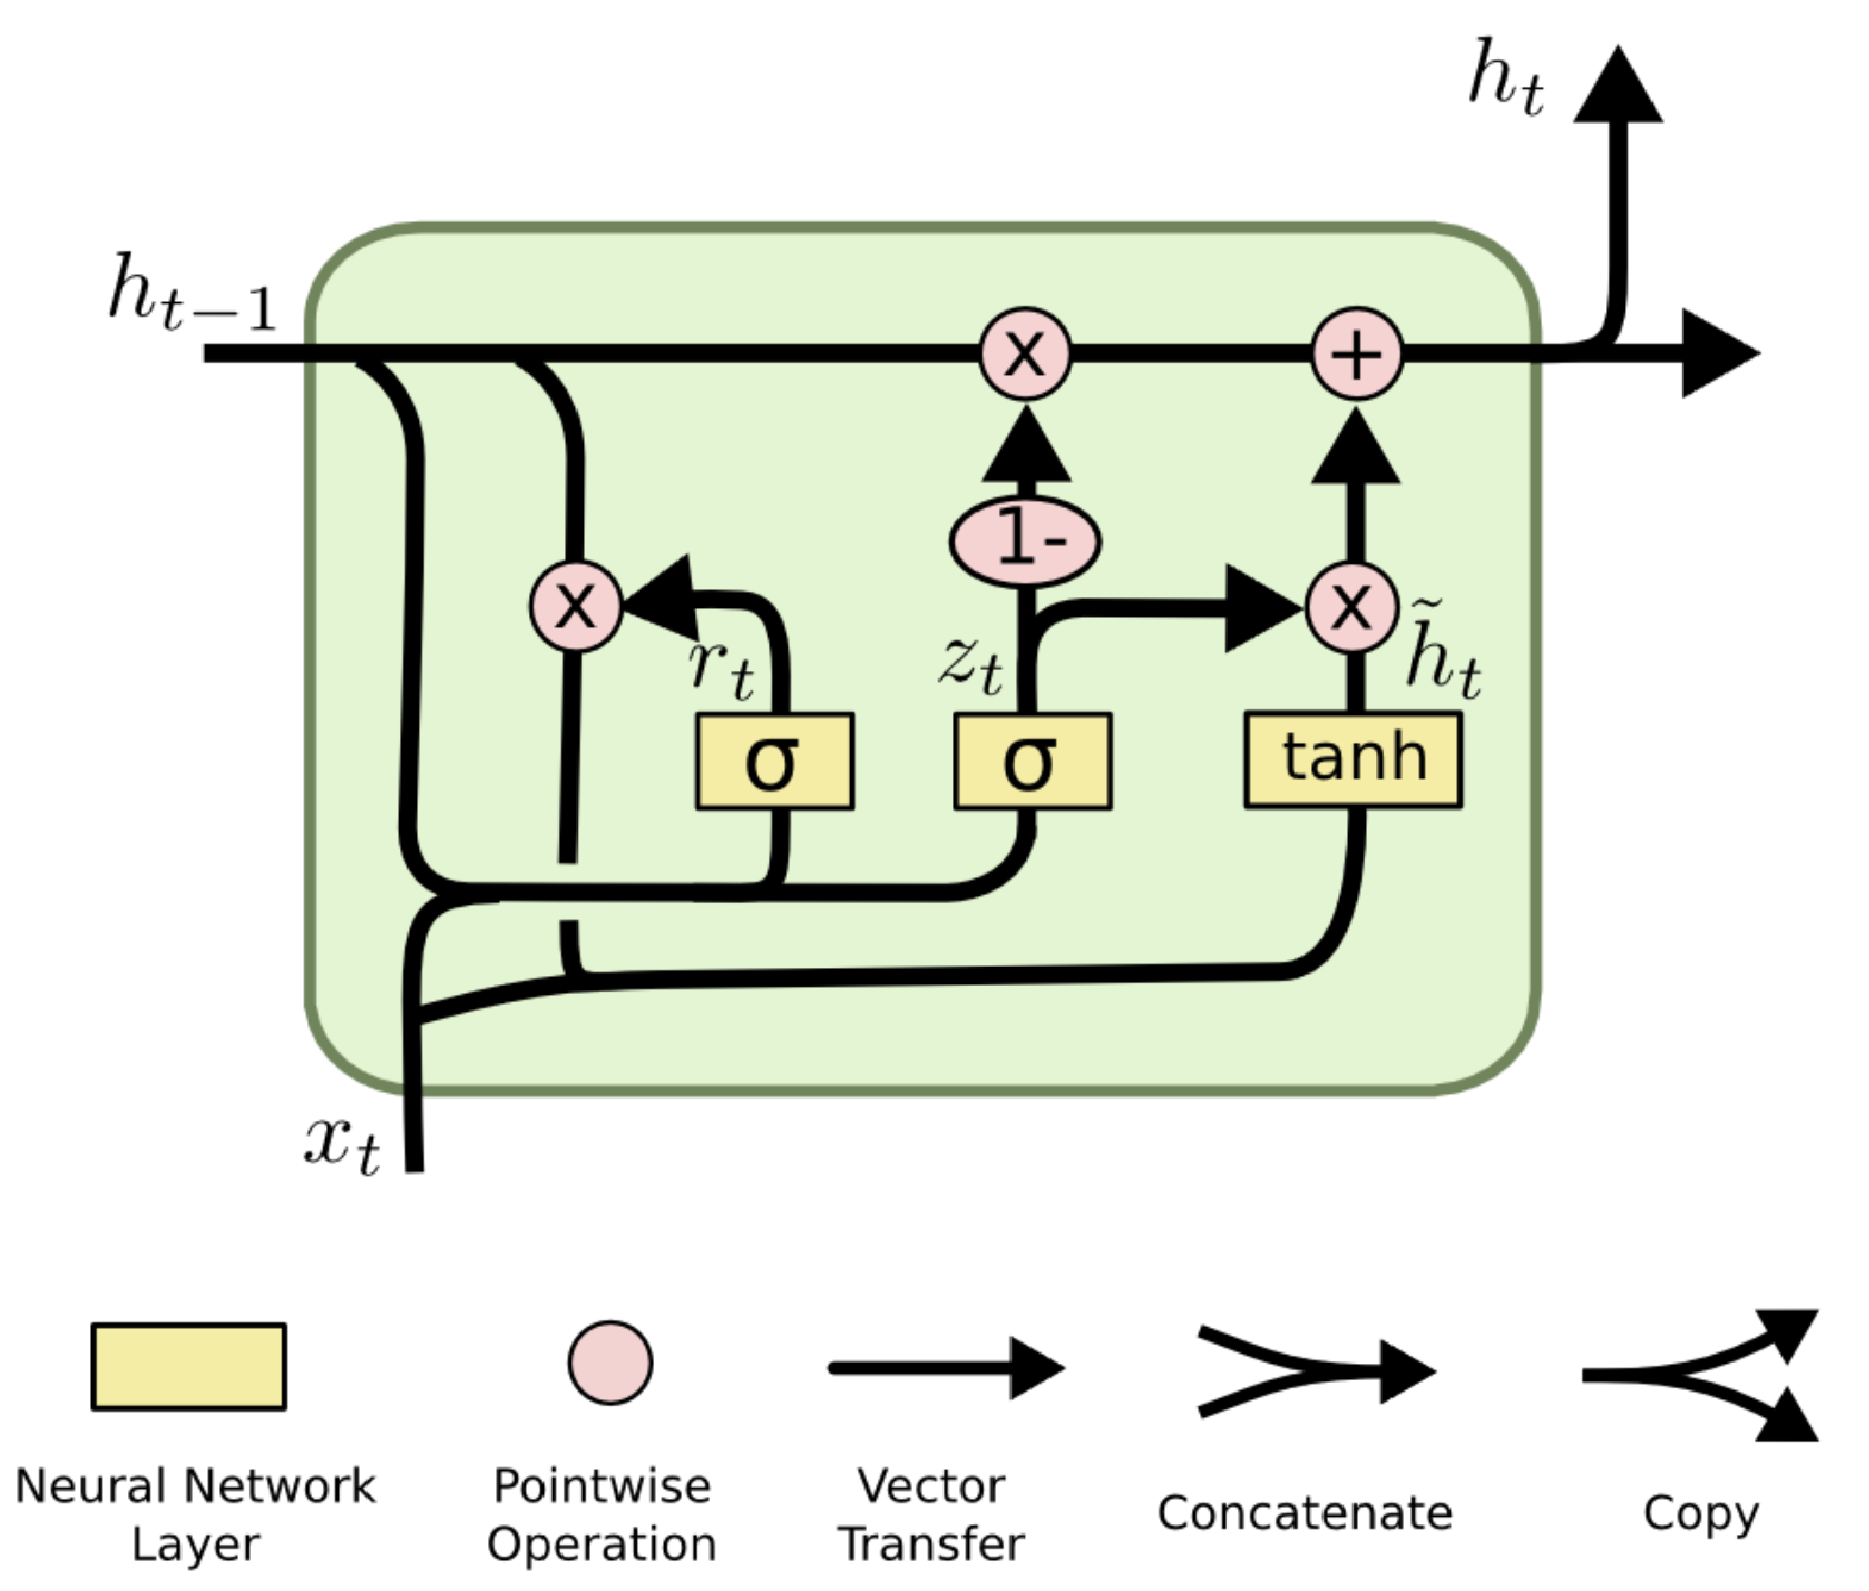
\includegraphics[width=0.6\textwidth]{gated_recurrent_unit.pdf}
\caption{An illustration of the Gated Recurrent Unit (GRU) architecture, from the online post by \citet{olah2015understanding}.}
\label{02_fig:gru_architecture}
\end{figure*}

This can be modeled by a variety of deep learning architectures in the \textit{encoder-decoder} framework. Specifically, we first encode the dialogue history $x^i_{<t}$ with an \textit{encoder}, followed by a \textit{decoder} to predict $x^i_{t}$. There are multiple architectures that can handle this, including LSTM \citep{hochreiter1997long}, GRU \citep{cho2014properties} and Transformers \citep{NIPS2017_3f5ee243}. Arguably, the simplest architecture is the GRU (short for ``Gated Recurrent Units''), which is illustrated in Figure \ref{02_fig:gru_architecture}. This is a type of recurrent neural network, whose hidden state $h_t$ at position $t$ is dependent on the input $x_t$ and previous state $h_{t-1}$ and computed in the following way:\footnote{Note that we abbreviate the superscript $i$ (indicating the ID of the dialogue sequence) for simplicity.}

\begin{align*}\label{eqt:gru}
& z_t = \sigma \,(W_z \cdot (h_{t-1} \odot x_t)) \\
& r_t = \sigma \,(W_r \cdot (h_{t-1} \odot x_t)) \\
& \tilde{h}_t = \mathrm{tanh} \,(W \cdot ((r_t * h_{t-1}) \odot x_t)) \\
& h_t = (1 - z_t) * h_{t-1} + z_t * \tilde{h}_t
\end{align*}

\noindent
Here, $W_z$, $W_r$ and $W$ represent learnable matrices, $\cdot$ represents the matrix (dot) product, $\odot$ represents the vector concatenation, and $*$ the elementwise (Hadamard) product. Crucially, $h_t$ is a linear interpolation of the previous state $h_{t-1}$ and the updated state $\tilde{h}_t$ (based on $x_t$) to address the \textit{vanishing gradient problem} \citep{bengio1994learning}.

As a last remark, we can easily incorporate (non-linguistic) dialogue context into the problem formulation. To be specific, let $D = \{(d^1, c^1), (d^2, c^2), ..., (d^{|D|}, c^{|D|})\}$ represent the dialogue corpus containing the additional dialogue context $c^i$. Then, the learning objective would be to minimize the following loss function:
%
\begin{equation}\label{eqt:sequence_to_sequence_with_context}
L(\theta) = \sum_{i = 1}^{|D|} \sum_{t = 1}^{|d^i|} - \log p(x^i_t | x^i_{<t}, c^i, \theta)
\end{equation}
%
This can be handled by a straightforward extension of the encoder, e.g. using Convolutional Neural Networks (CNN) to encode visual contexts \citep{NIPS2012_c399862d,xu2015show}. Due to its flexibility, scalability and generality, this approach has been applied in a wide variety of tasks, including traditional task-oriented dialogues \citep{bordes2017learning,wen-etal-2017-network,ham-etal-2020-end}, multi-modal dialogues \citep{das2017visdialrl,Kottur_2018_ECCV,NEURIPS2019_c74d97b0}, non-cooperative dialogues \citep{lewis-etal-2017-deal,DBLP:conf/icml/YaratsL18,li2020noncollaborative} and non-goal-oriented dialogues \citep{vinyals2015neural,adiwardana2020towards,roller-etal-2021-recipes}.\\

In both approaches, common ground is represented as the \textit{dialogue state} of the systems: namely \textit{structured} representations (such as frames and data-flow graphs) in the first approach and \textit{learned} representations (e.g. the hidden state $h_t$) in the second approach. Due to this difference, the first approach tends to perform more reliably in schematic traditional dialogue tasks \citep{takanobu-etal-2020-goal}, while the second approach is preferred in other domains. Since our proposed tasks are non-schematic and require dealing with non-linguistic (visual) contexts, we generally focus on the second approach (end-to-end dialogue models) as our baselines in this thesis.

\section{Symbol Grounding}
\label{02_sec:symbol_grounding}

\textit{Symbol grounding} is another primary competence of natural language, which refers to the process of connecting symbolic language to the physical world \citep{harnad1990symbol}. In this section, we first discuss the important relations between common grounding and symbol grounding with respect to \textit{natural language acquisition} \citep{tomasello2009constructing}. Secondly, we focus on computational approaches to \textit{spatio-temporal grounding} and review the emerging literature in the fields of CV and NLP. 

\begin{figure*}[t!]
\centering
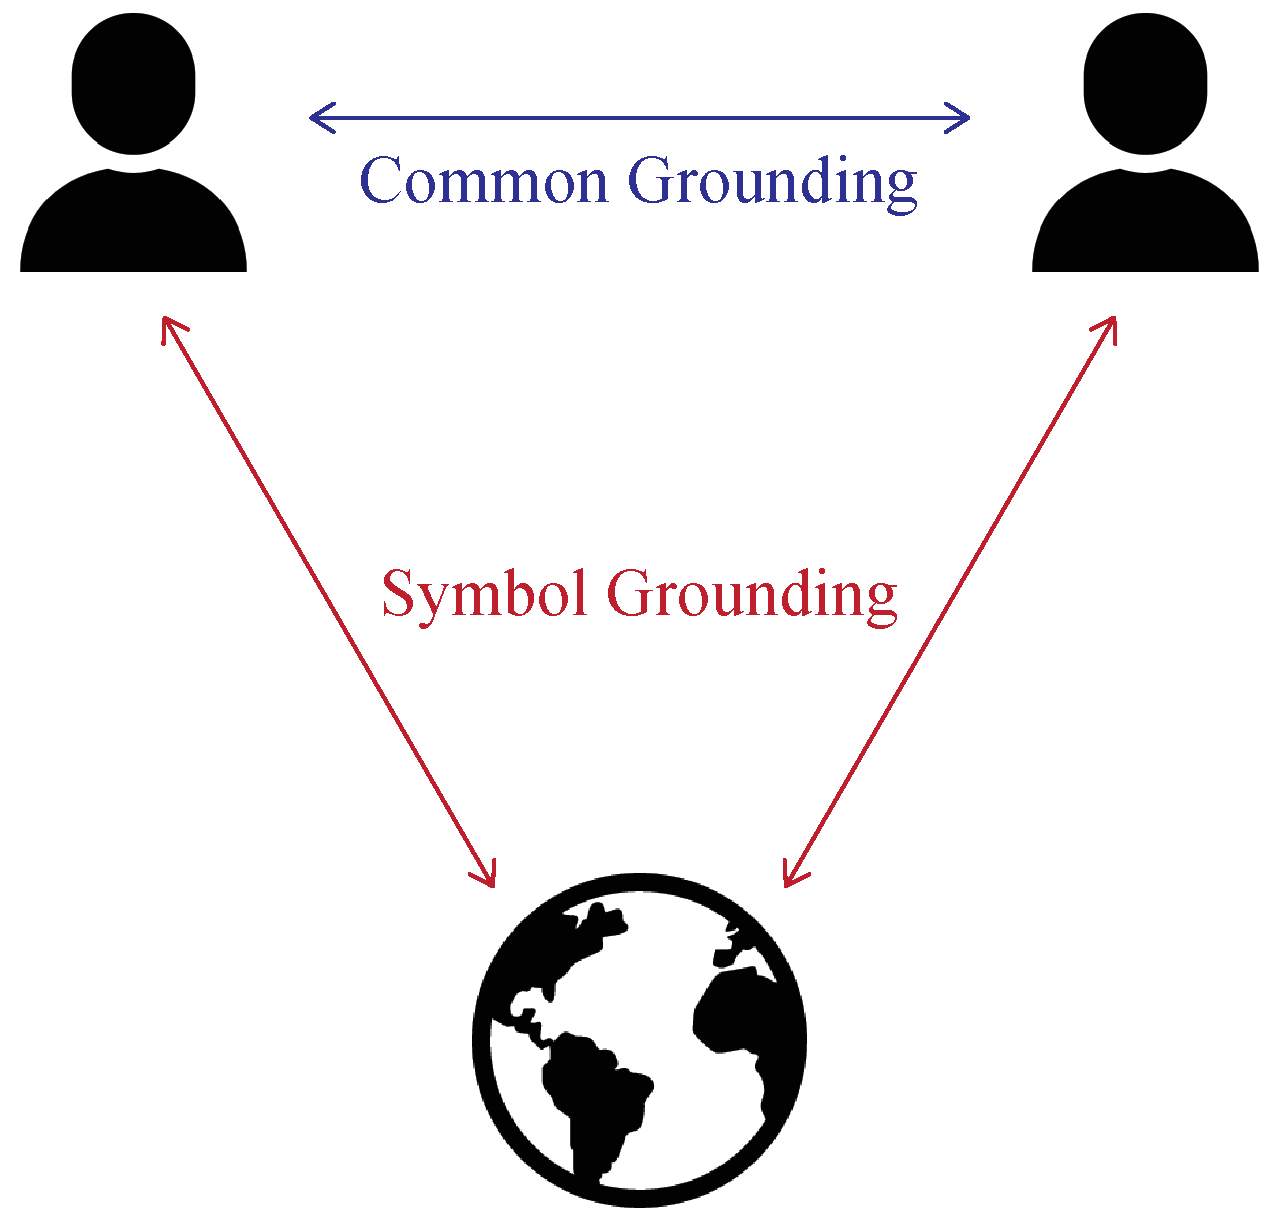
\includegraphics[width=0.5\textwidth]{triadic_relations.pdf}
\caption{The triadic relations of common grounding and symbol grounding.
}
\label{02_fig:triadic_relations}
\end{figure*}

\subsection{Language Acquistion}
\label{02_subsec:language_acquisition}

The meaning of language cannot be defined by the language itself, as it would lead to an endless circular definition: instead, it must be somehow connected to the physical world in the right way \citep{harnad1990symbol}. At the same time, we cannot use language in an arbitrary way if we were to communicate with each other: the usage of language must become a \textit{convention} through the process of common grounding \citep{lewis1969convention}. These two requirements form an intricate triadic relationship in terms of constructing and acquiring natural language, as depicted in Figure \ref{02_fig:triadic_relations}.

This relationship has been noticed and investigated in a variety of literature. In developmental psychology, the establishment of \textit{joint attention} (mutual recognition of an external entity) has been regarded as a crucial basis for first language acquisition \citep{clark2001grounding,tomasello2009constructing}: this is a representative example where common grounding meets symbol grounding. In the fields of linguistics and AI, there has been an intense debate over the schools of nativism, empiricism and culturism \citep{Chomsky1957-CHOSS-2,elman1996rethinking,steels1997synthetic}. For instance, the naming of color in human language may be affected by the innate structure of our perception, the physical world and environments we experience, or the requirements as a social tool for communication \citep{Steels2005coordinatingPG}. The converging view seems to suggest that all of these perspectives matter, complexly involving innate human structures, symbol grounding and common grounding \citep{larsson2018grounding}.

On the other hand, the NLP community has been predominantly focusing on the study of static corpora. Such corpus-driven approach originates in the seminal work of Penn Treebank \citep{marcus-etal-1993-building} and often validated on the account of the \textit{distributional hypothesis}, known for the famous quote from \citet{firth1957synopsis} -- ``you shall know a word by the company it keeps''. This approach has been successful to a remarkable extent: state-of-the-art models achieve near human-level performance on a range of natural language understanding benchmarks \citep{wang-etal-2018-glue,devlin-etal-2019-bert}, even in the challenging few-shot settings \citep{NEURIPS2020_1457c0d6}. However, upon deeper inspection, their linguistic abilities often turn out to be brittle and shallow, as we've seen in the case with BlenderBot (c.f. Section \ref{02_subsec:tasks_and_datasets}). Consequently, increasing works caution that language acquisition cannot be realized only from its forms (corpora) and requires interaction with the real world and other humans \citep{bisk-etal-2020-experience,bender-koller-2020-climbing,benotti-blackburn-2021-grounding}. 

Building upon these backgrounds/observations, we make an important contribution to study the triadic relationship of common grounding and symbol grounding in a minimal yet advanced setting. To be specific, we focus on the primary notion of \textit{joint attention} and incorporate realistic factors of human dialogues in the physical environments: namely \textit{continuity}, \textit{partial-observability} and \textit{dynamics}.


\subsection{Spatio-Temporal Grounding}
\label{02_subsec:spatio_temporal_grounding}

While symbol grounding encompasses all conceivable connections between language and the physical world, one principal connection is made on the dimensions of space and time. This type of connection, which we refer to as \textit{spatio-temporal grounding}, has been an important subject of study at the intersection of CV and NLP.
\\

\noindent
\textbf{Visual Grounding Tasks}\quad
Vision-language grounding has been a longstanding goal in the fields of CV and NLP. This is fundamental for developing systems that can not only \textit{speak} but also \textit{perceive} and \textit{act} in the physical world, just as we normally do. Such technology is also crucial for making information accessible to the visually-impaired, e.g. by automatically rendering visual contents to natural language descriptions.

One representative task of visual grounding is the \textit{visual question answering (VQA)} task. This requires the models to answer correctly to the questions (information requests) related to the visual context, including images \citep{antol2015vqa,hudson2019gqa} as well as videos \citep{lei-etal-2018-tvqa,lei-etal-2020-tvqa}. In the \textit{visual captioning (VC)} task, the goal is to provide the descriptions of salient objects, events, background, etc in a given scene through natural language \citep{xu2015show,hossain2019comprehensive}. Finally, in \textit{visual dialogues}, the task is extended to an interactive setting, typically involving both the \textit{reactive} aspects of VQA and \textit{proactive} aspects of VC \citep{das2017visual,de2017guesswhat,alamri2019audio}.

However, realistic visual contexts are often unbalanced and lack diversity in terms of spatio-temporal relations. For instance, in natural photographs, a dog would most likely be \textit{under} a tree rather than \textit{on top of} a tree. In natural videos, a book would typically \textit{fall off} the shelf but not \textit{float up} to the shelf. When such biases exist, the spatio-temporal attributes and relations may be identifiable based on superficial clues only, e.g. by simply recognizing the object categories (\textit{dog}, \textit{tree}, \textit{book}, \textit{shelf}, etc) \citep{goyal2017making,cirik-etal-2018-visual}.

\begin{figure*}[t!]
\centering
\begin{minipage}{.5\textwidth}
  \centering
  \includegraphics[width=.93\textwidth]{clevr_sample.pdf}
\end{minipage}%
\begin{minipage}{.5\textwidth}
  \centering
  \includegraphics[width=.92\textwidth]{nlvr_sample.pdf}
\end{minipage}
\caption{Example questions from the CLEVR dataset \citep{johnson2017clevr} (left) and the NLVR dataset \citep{suhr2017corpus} (right).
}
\label{02_fig:clevr_nlvr_sample}
\end{figure*}

One solution to circumvent this issue is to use synthetic visual contexts. As an illustration, we show example instances from CLEVR \citep{johnson2017clevr} and NLVR datasets \citep{suhr2017corpus} in Figure \ref{02_fig:clevr_nlvr_sample}. In these datasets, the entity attributes and relations are restricted to preliminary concepts but randomly sampled in a fully controlled manner. This way, their \textit{combinatorial} variety is maximized while reducing exploitable biases, requiring genuine understanding and compositional generalization \citep{Fodor1988ConnectionismAC,Lake2018GeneralizationWS}. Furthermore, the controllability of the context allows for various in-depth analyses of complex models, e.g. error analyses and \textit{causal} analyses through direct intervention \citep{pearl2009causality,pearl2018book}.

While these two approches have complementary strengths and weaknesses, we generally follow the second line of research (based on synthetic contexts) to maximize the diversity of spatio-temporal expressions and enable faithful evaluation and diagnosis of spatio-temporal grounding.
\\

\noindent
\textbf{Spatio-Temporal Language}\quad
Finally, spatio-temporal language has a long history of research as well. In computational linguistics, annotation frameworks have been proposed to capture the events, time and temporal relations expressed in natural language, e.g. in news articles \citep{pustejovsky2003timeml,ning-etal-2018-multi}. The annotation of spatial language has also been attempted to capture the information related to locations, directions, topological relations and motions \citep{pustejovsky2011iso,dan-etal-2020-spatial}. The recognition of such spatio-temporal information plays a fundamental role in natural language comprehension \citep{zwaan1998situation} as well as pratical applications such as information extraction and text mining \citep{banko2007,Aggarwal2012MiningTD}.

In the CV community, one of the most popular representations of spatio-temporal information is based on the \textit{scene graphs} \citep{johnson2015image,krishna2017visual}. In this approach, spatio-temporal attributes and relations are captured in the \textit{predicate-argument structure}, as shown in Figure \ref{02_fig:scene_graph}. This allows for a natural mapping from spatio-temporal language to \textit{regions} (e.g. object boundaries) in the visual scenes.

\begin{figure*}[t!]
\centering
\includegraphics[width=0.6\textwidth]{scene_graph.pdf}
\caption{An example of the scene graph representation from \citet{johnson2015image}.}
\label{02_fig:scene_graph}
\end{figure*}

However, existing works mostly focus on \textit{monologues} rather than dialogues, ignoring the important intersection between symbol grounding and common grounding. In dialogues, speakers often have incomplete/asymmetric information, requiring collaborative coordination on the semantics, references, \textit{frames} of references, etc: for instance, the referent of the speaker may not be visible/groundable for the listener. To address such issues, interlocutors often rely on \textit{modifications} to express precise information \citep{paradis_2008} and \textit{ellipses} to make conversation efficient. 

These factors can make the application of existing approaches (e.g. annotation frameworks and scene graphs) nontrivial, yet mostly ignored in the prior literature (e.g. \citealt{elliott-keller-2013-image}). In this thesis, we explicitly take into account such complexities and propose a simple yet challenging testbed of spatio-temporal language in interactive conversations.
